\documentclass[10pt,twocolumn]{article}
\usepackage[margin=2.3cm]{geometry}
\usepackage{float}
\restylefloat{table}
\usepackage{cite}
\usepackage{hyperref}
\usepackage{graphicx}
\usepackage{authblk}
\usepackage[latin1]{inputenc}
\usepackage{subfigure}
\usepackage{listings}
\usepackage{pbox}
\usepackage{float}
\usepackage{fancyvrb}
\usepackage{multirow}
\usepackage{changebar}
%\usepackage{url}
\usepackage{array}
\usepackage{color}
\usepackage{rotating}
\usepackage{titlesec}
\restylefloat{figure}
\usepackage{epstopdf}
\usepackage{colortbl}
\usepackage{setspace}
%\usepackage{breakurl}
\usepackage[belowskip=-5pt]{caption}
\singlespacing
\usepackage{amsmath}
\usepackage{amssymb}

\newcommand{\attGood}{\ensuremath{\checkmark}}
\newcommand{\attBad}{\ensuremath{\times}}

\newcount\Comments  % 0 suppresses notes to selves in text
\Comments=1   % TODO: set to 0 for final version

% for comments
\usepackage{color}
\definecolor{darkgreen}{rgb}{0,0.5,0}
\definecolor{purple}{rgb}{1,0,1}
% \kibitz{color}{comment} inserts a colored comment in the text
\newcommand{\kibitz}[2]{\ifnum\Comments=1\textcolor{#1}{#2}\fi}
% add yourself here:
\newcommand{\joao}[1]{\kibitz{red}      {[JOAO: #1]}}
\newcommand{\jianneng}[1]{\kibitz{cyan}     {[JIAN: #1]}}
\newcommand{\team}[1]  {\kibitz{purple}   {[TEAM: #1]}}


\begin{document}
\title{{\bf Recoverable Virtual Memory: A Simple Solution for Data Replication}}
\author{
    Nathan Pemberton, Howard Mao, Jo\~{a}o Carreira
}
\maketitle

%%%%%%%%%%%%%%%%%%%%%%%%%%%%%%%%%%%%%%%%%%%%%%
\begin{abstract}
In large-scale distributed systems failures are the norm rather than the exception. 
To cope with hardware and software failures developers make use of two main techniques: 1) persisting data to a non-volatile storage device such as a hard drive, or storing data in a distributed storage system such as a DBMS or key-value store. 
While the first approach is slow and leaves the program's progress disk-bound, the second approach requires the usage of complex APIs that require serialization of user's data structures.

To solve this problem we built Nephele, a framework that provides replication of in-memory data structures efficiently through a simple API. 
Nephele replicates a program's data to a remote node through RDMA providing snapshots of program's data with latency on the order of a few microseconds.
The framework provides a transactional interface to users that guarantees atomicity and durability even in the face of failures.

Nephele consists of two layers: a transactional layer for recoverable virtual memory (RVM) and a remote memory storage layer. The user-facing transaction layer provides an API consisting of 15 methods and is responsible for detecting changes and replicating changes at commit time. The remote memory storage layer is responsible for storing user's data in a remote node over RDMA. For this layer we have implemented two backends: one using a custom RDMA protocol with a custom server, and one using RAMCloud, a RDMA-optimized key-value store.

To demonstrate the flexibility and performance of our system we applied our framework to three applications: a genomic assembly program, an in-memory file system and a vector-matrix multiplication application.
We show that our framework provides data replication with negligible overhead.


\end{abstract}

%\vfill
%\eject
%%%%%%%%%%%%%%%%%%%%%%%%%%%%%%%%%%%%%%%%%%%%%%
\section{Introduction}
As the number of nodes in distributed systems increases, failures become the
rule, not the exception. Because of this, it is important to be able to recover
from crashes quickly.  In addition, the application should not be made
significantly more complicated by the addition of recovery code.

While it would be overly ambitious to try and solve this entire goal, we propose
a tool that could simplify such a solution by providing the ability to replicate
the application's working state to another failure domain. In this report, we
present an implementation of Recoverable Virtual Memory (RVM), an API that
allows the programmer to easily add state checkpointing and recovery to their
application. RVM operates by detecting modifications to recoverable memory
regions and replicating the memory to a remote node.

The proliferation of high-performance RDMA and future disaggregated memory
systems offer an opportunity to perform this replication efficiently. For
example, the FireBox warehouse-scale computer (an ASPIRE lab project) will have
a central pool of universally accessible DRAM and non-volatile memory. Currently
there is no FireBox hardware to experiment with, but we do have an infiniband
based cluster (Firebox-0). So far, we have implemented two backends, one using
the Infiniband RDMA API and one using the Ramcloud key-value store.

\subsection{Current Solutions}
The need to preserve critical data in the event of a hardware failure is not
new. There are a number of popular methods of addressing this problem. One is to
checkpoint the entire operating system process using a tool like the Berkeley
Lab Checkpoint Restart library\cite{BLCR} or Condor\cite{Condor}). Process
checkpointing is appealing because it requires little to no changes in the
application. For this convenience, the technique sacrifices efficiency. All data
must be checkpointed, not just the critical state, and operating system state
must be quiesced. A common practice to avoid avoid copying the entire program
state is to manually serialize critical data structures and write them to a
file. While, in theory, this technique copies the minimum amount of data, in
practice it can be difficult to identify which state has actually changed. The
user is forced to pessimistically replicate most critical state on each
checkpoint. Manual serialization also leads to significant increases in code
complexity. Each data structure must have two definitions, one for on-disk and
the other for in-memory. Maintaining this serialization code can be
time-consuming and error-prone. Finally, databases are commonly used to
replicate critial state.
Databases provide clean transactional semantics that can be appealing for
high-availability applications. Databases, however, often have a complex
interface that requires manual serialization. They also provide more features
than are required for state replication, which leads to poor performance.

\subsection{RVM Interface}
The RVM interface is designed to be as unobtrusive as possbile. Users should be
able to preserve just their critical state without worrying about re-writing
pointers or packing data into a file. To do this our framework requires only
that the user identify which memory is considered critical, and identify points
of consistency in their code. By marking a point of consistency the user
certifies that, if the program we're to restart with the critical memory in the
current state, the program would be able to continue execution. Critical state
is identified by allocating it from a special recoverable malloc function and
consistency points are identified through a transactional interface. Users may
also save a special \bf{user\_data} pointer that survives failures. This pointer
typically stores a state structure that can address the recoverable state in an
application-dependent fashion. Table \ref{RVM API} lists the entire required API.

\tabular{ | l | l | }
rvm_cfg\_\[create/destroy\]() & Initialize the system and recover memory if
needed.
\\
\hline rvm\_\[alloc/free\]() & Allocate a region of recoverable memory. \\
\hline rvm_txn\_\[start/commit\]() & Mark a point of consistency in the program.
\\
\hline rvm\_\[set/get\]\_usr\_data() & Register a pointer to your state. \\
\end{tabular}

In practice, of course, it is not this simple. Code must be written in such a
way that recovery is possible. In addition, while critical local state is
preserved, external state (like open files or sockets) is not. RVM is intended
as a low-level library that can be exploited by more full-featured recovery
libraries. An analogous relationship can be seen in the GASNet \cite{GASNET}
library which can be used directly, but is really intended as a low-level
interface for global address space langauges.

\section{Design}
\subsection{The RVM API}

The RVM layer is responsible for implementing the custom allocator and
identifying changes to memory. It is also responsible for tracking commit
points.

\subsubsection{The Block Table}
The RVM layer thinks in terms of \emph{blocks}, fixed-sized regions of
memory that are persisted atomically. Most functionality is based around the
\emph{block table}, a persistent data structure that keeps track of each
allocated block in the system. This table is replicated using the same
mechanism as any other recoverable memory. Like a filesystem master boot record,
the first page of the block table is always stored with a constant identifier
in the RMEM layer. After that, the block table is self-describing and can be
recovered using the mechanisms described below.

Each entry in the block table contains a local address where the active block
lives on the client and a remote identifier that can be used to identify the
block in the RMEM layer. 

\subsubsection{Initialization and Recovery Procedure}

When \verb|rvm_cfg_create()| is called the first time, it initializes the block
table to an empty state and persists it in the RMEM layer. When recovering,
\verb|rvm_cfg_create()| fetches the first block of the block table from the
RMEM layer. The block table is walked from start to finish, fetching each block
as it goes. Even if the block table takes up multiple blocks, each one is
fetched in order, ensuring that all data can be found eventually. When RVM
fetches a remote block, it must ensure that it is loaded to the same address it
was at before failure, otherwise pointers in the data would no longer be valid.
The original address is read from the block table and then allocated using the
\emph{mmap()} system call. To ensure that these addresses are always available,
RVM requires that any OS address space layout randomization be disabled, and
that \verb|rvm_cfg_create()| be called before any other local allocations.

\subsubsection{Allocation}

To ensure that memory is recoverable, the user must allocate it using a special
\verb|rvm_alloc()| function. The \verb|rvm_alloc()| function allocates memory
both locally and on the remote node. Any modifications to the local pages
allocated by \verb|rvm_alloc()| are automatically detected and copied to the
remote node at commit time. Detection is achieved through the use of
\emph{mprotect()}, a Linux system call that can be used to make the application
take an interrupt whenever a page is written. Our custom interrupt handler
then marks the page as changed, removes the memory protection and returns. This
means that RVM needs to be involved only in the first modification to a page.

\subsubsection{Marking a Point of Consistency}

The user is required to identify points in their code where the state of
recoverable memory is considered \"consistent\". This means that recovery is
possible from that particular state. \verb|rvm_txn_commit()| can be called at
these points to ensure that memory is atomically persisted. Upon entering
\verb|rvm_txn_commit()|, RVM goes through the list of changed pages and copies
them to a shadow page in the RMEM layer. This ensures that a consistent version
of memory is always available, even if the client crashes during checkpointing.
When all the pages have been copied, an \verb|atomic_commit()| function
(provided by the RMEM layer) is called to persist the changes.



\subsection{The Remote Memory Layer}

Underlying the RVM API is the remote memory (RMEM) layer, which provides the
basic operations that RVM uses to communicate with the backing data store.
The essential operations in the RMEM layer are \texttt{malloc()},
\texttt{free()}, \texttt{put()}, \texttt{get()}, and \texttt{atomic\_commit()}.

The \texttt{malloc()} function allocates memory in the backing store.
The function arguments include the number of bytes to allocate as well as
a unique tag that is associated with that memory region. If the tag has not
already been taken, \texttt{malloc()} allocates a new memory region and returns
the starting address. If a memory region with that tag already exists, the
starting address of the previously allocated region is returned.

The \texttt{free()} function takes a tag as its argument and frees the memory
region associated with that tag.

There are also \texttt{multi\_malloc()} and \texttt{multi\_free()} functions
which allocate and free multiple memory blocks. Depending on the backend,
these functions might coalesce \texttt{malloc()} and \texttt{free()} requests
in order to decrease the number of round trips to the backing store.

The \texttt{put()} and \texttt{get()} functions copy data to and from the
backing store, respectively. These operations are not atomic, so the RVM
layer always performs puts and gets onto a shadow page and then copies the
data to the real page using \texttt{atomic\_commit()}.

As mentioned before, \texttt{atomic\_commit()} takes an array of source tags
and an array of destination tags. It instructs the server to copy the data
in the source memory regions to the destination regions. This copying is
done atomically, so there is no danger of only a portion of the pages
being copied due to the client crashing.


\subsection{Infiniband Backend}

Our primary backend uses Infiniband Remote Direct Memory Access (RDMA) to talk
to a server managing a large pool of memory. At startup, the remote memory
server maps in a large block of system memory. The server then listens for
connections over the Infiniband fabric. When a client connects, the server
pins the memory in the page table and registers it with the infiniband drivers.
Registering with the infiniband drivers provides a local key and a remote key.
The server transmits the remote key and starting address to the client.
This allows the client to perform one-sided RDMA operations to the remote
memory without the server's mediation.

The \texttt{put()} and \texttt{get()} commands are implemented using one-sided
RDMA writes and reads. The other commands are implemented using two-sided sends
and receives. For these commands, the client and server each allocate two
message structs: one for sends, and one for receives. In a two-sided
transmission, the recipient first posts a receive request to the Infiniband
driver. This receive request specifies the local key and address of the receive
struct. When the sender posts a corresponding send request using the local key
and address of its send struct, the infiniband drivers copy the data from the
sender's send struct to the recipient's receive struct and notify sender and
recipient of the operation.

\begin{figure}
    \includegraphics[width=0.9\linewidth]{ib-backend-arch.pdf}
    \caption{IB Backend Architecture}
    \label{fig:ib-backend-arch}
\end{figure}

\subsubsection{Allocation}

The \texttt{malloc()} operation is implemented by sending an ALLOC request to
the server. When it receives this request, the server will allocate a block of
memory form the memory pool and mark it with the given tag.  The server then
sends a MEMRESP message back to the client containing the starting address of
the allocated block.

The \texttt{free()} operation is implemented by sending a TXN\_FREE request to
the server. A key feature of the IB backend is that the server does not
immediately perform a free operation when it receives the TXN\_FREE message.
Instead, it puts the free operation in a queue, which will be processed during
an atomic commit. This way, the free operation is transactional. Once the
server receives the message and queues the free operation, it sends a TXN\_ACK
message back to the client, allowing the client to send another command.

There are also MULTI\_ALLOC and MULTI\_TXN\_FREE requests which can encode up
to 20 allocation or free requests (this number if configurable at compile
time). The server responds to a MULTI\_ALLOC request with a MULTI\_MEMRESP
response, which contains an array of addresses, one for each tag in the
MULTI\_ALLOC request. The server responds to MULTI\_TXN\_FREE with a TXN\_ACK.

\subsubsection{Commit}

The \texttt{atomic\_commit()} operation involves two different message types.
The first is the MULTI\_TXN\_CP message, which instructs the server to copy a
set of source blocks to a set of destination blocks. However, as with
TXN\_FREE, the copy does not occur immediately. When the client sends the
server a TXN\_GO request, the server performs all requested copies and frees.
In our failure model, we assume that the server will not crash. So even if the
client crashes after sending TXN\_GO, the copies and frees will still be
performed to completion. If the client crashes before sending TXN\_GO, all of
the outstanding copy and free requests will be flushed and no changes will
occur.

\subsubsection{Recovery}

If a client reconnects after a crash, the IB server transmits the tag to
address mappings left over from the previous run to the client. The mappings
are transmitted to the client in groups of twenty through TAG\_ADDR\_MAP
messages. The client acknowledges each TAG\_ADDR\_MAP message with a
STARTUP\_ACK message.


\subsection{Ramcloud Backend}

% Ramcloud Backend

\begin{figure}[t!]
\begin{center}
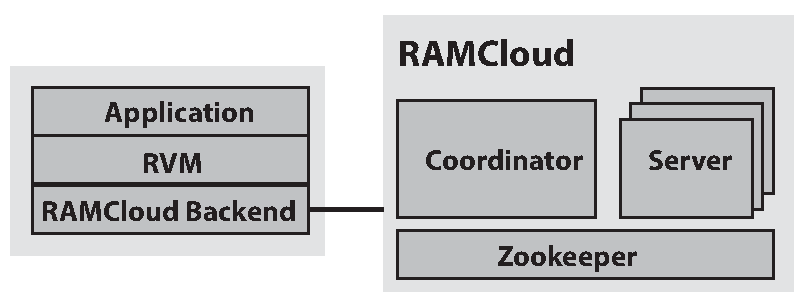
\includegraphics[scale=0.60]{graphs/ramcloud_backend_design2.pdf}
\end{center}
\caption{RAMCloud backend layer operating along side RAMCloud.}
\label{fig:ramcloud_backend_design}
\end{figure}

\begin{figure}[t!]
\begin{center}
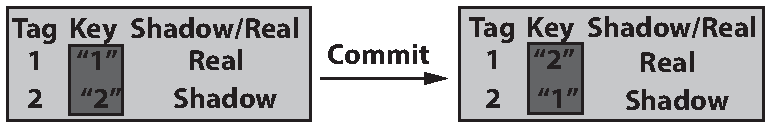
\includegraphics[scale=0.60]{graphs/ramcloud_backend_commit.pdf}
\end{center}
\caption{Diagram of tag/key mapping transformation during commit for a single memory region.}
\label{fig:ramcloud_backend_commit}
\end{figure}

To investigate the performance and suitability of a key-value store as a block device we developed a software layer on top of RAMCloud, a low-latency key-value store.
In RAMCloud, blobs of memory (values) are identified by keys (strings). When running RAMCloud is composed of three main executing instances: a coordinator, a server and Zookeeper (see Figure~\ref{fig:ramcloud_backend_design}).
Each server is responsible for storing and serving data (values). The coordinator is responsible for keeping track of all servers alive and for keeping track of where data is stored in the system.
A Zookeeper instance is used for leader election and for storing configuration data.

Because RAMCloud's data is reference by keys (string) this layer keeps a map structure that associates each tag to a key. This means that each recoverable memory region can be uniquely identified by a key.

To provide atomicity and durability of the tag/key mapping, this backend keeps a special entry in RAMCloud with each tag-key association. This table is read each time the software layer is started and written once for each commit. Because this entry can be atomically written with a {\emph put} operation, we can provide very efficient atomic writes.

Th RMEM's layer operations are implemented in the following way:

\paragraph {\bf Connect} During connection the backend creates a RAMCloud client instance that is responsible for estabilishing a connection to the RAMCloud server.
If this is not the first time this connection is performed, i.e., if the client is under recovery, the backend recoveres each tag-key mapping.
Otherwise, this layer initializes a RAMCloud table and stores an empty master entry in the RAMCloud's server.
\paragraph{\bf Allocate} During allocation, first the backend creates a key that identifies the memory being allocated in the RAMCloud server. Secondly, RAMCloud initializes
\paragraph{\bf Write} To write a memory region (identified by a tag) the backend fetches the tag's corresponding key and issues a {\emph put } operation with that key and corresponding data.
\paragraph{\bf Read} Likewise, to read a memory region the backend issues a {\emph get} operation with the tag's corresponding key. The data read from RAMCloud is copied to the final destination.
\paragraph{\bf Commit} To perform commit, the backend constructs a new master entry where each tag points to the key of the shadow memory being commited (see Figure~\ref{fig:ramcloud_backend_commit}). Likewise, the tag for each of the shadow
memory regions is made to point to the key of the old memory region (rephrase). Once this master entry is constructed in the backend, it is written atomically to RAMCloud.
\paragraph{\bf Disconnect} To disconnect, the backend clears the main data structures (e.g., local tag-key map).

Our design is simplified by the fact that our framework only replicates data to a single node. This means that we do not have to coordinate replicas.


\section{Evaluation}
\subsection{Micro Benchmarks}

We used micro-benchmarks to test the performance of RVM commits and RVM
recovery. To test commits, we allocated a number of pages, made modifications
to each one of them, and measured the time it took for \verb|rvm_txn_commit()|
to complete. To test recovery, we first allocate a number of pages and
close the connection to the server. We then restart the connection using the
recovery flag and time how long it takes \verb|rvm_cfg_create()| to complete.
When benchmarking the IB backend, we run three trials for each number of pages,
restarting the server after each trial.

\subsection{IB Backend}
Figure \ref{fig:ib-commit-ubm} shows the results of the commit micro-benchmark
using the IB backend. At the smallest page count, the commit time is around
150 microseconds. At 10K pages, the commit time has increased to 140 milliseconds.
As can be seen in the graph, the relation between page count and commit time
is fairly linear, with a slope of about 13.7 microseconds per page.

\begin{figure}[h]
    \caption{IB Commit Micro-Benchmark Results}
    \includegraphics[width=\linewidth]{graphs/commit-results-rm.pdf}
    \label{fig:ib-commit-ubm}
\end{figure}

Figure \ref{fig:ib-recovery-ubm} shows the results of the recovery
micro-benchmark using the IB backend. Recovery is quite a bit slower than
commit. Recovering a single page takes about 50 milliseconds, while recovering
10,000 pages takes more than 2 seconds. The relationship between number of
pages and recovery time is also not entirely linear.
The recovery time increases steadily until about 2000 pages, after which it
increases drastically. It is uncertain what is causing this sort of behavior,
as startup time involves a lot of different things, including the allocation
of local memory pages, receiving tag to address mappings from the server, and
copying data from the server.

\begin{figure}[h]
    \caption{IB Recovery Micro-Benchmark Results}
    \includegraphics[width=\linewidth]{graphs/recovery-results-rm.pdf}
    \label{fig:ib-recovery-ubm}
\end{figure}

\subsection{RAMCloud Backend}
\begin{figure}[t!]
\begin{center}
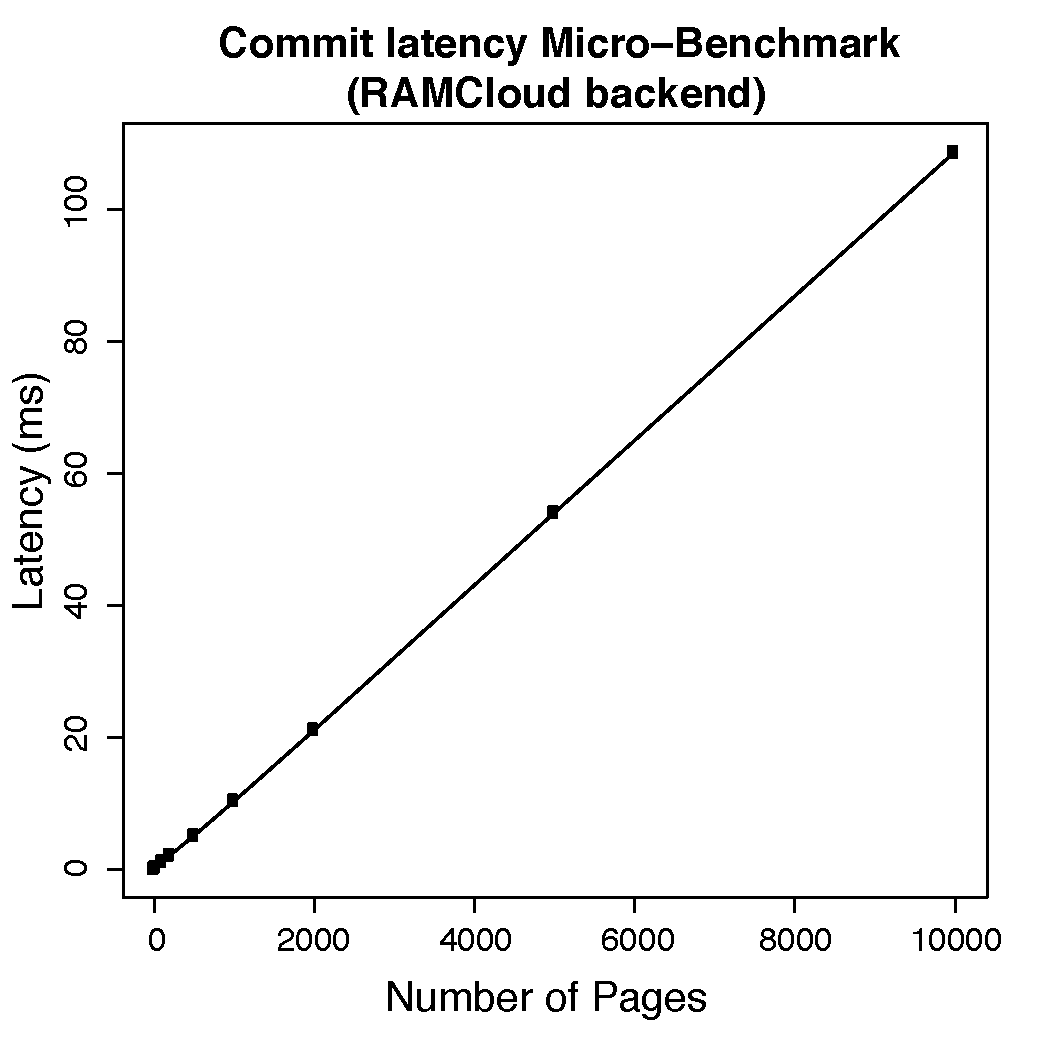
\includegraphics[scale=0.40]{graphs/commit_time_rc_latencies.pdf}
\end{center}
\caption{Commit time micro-benchmark when using the RAMCloud backend}
\label{fig:inmem_fs_design}
\end{figure}

Figure~\ref{fig:inmem_fs_design} shows the results of the commit micro-benchmark when using the RAMCloud backend. 
The end-to-end latency of a commit operation is dominated by the number of pages to be commited, as each page write requires a round-trip to the RAMCloud server.
The RAMCloud backend also needs to save the table that contains the mapping between tags and keys in, but this only requires one interaction with the server.
The RAMCloud backend requires roughly 10 microseconds to write a page to RAMCloud. As can be seen in the graph, the commit time grows linearly with the number of pages as expected.







\subsection{DGEMV}

% DGEMV
Our first attempt at making a realistic application recoverable was an
iterative dense matrix-vector multiply (DGEMV) code. This application
repeatedly multiplies a vector by a constant matrix. Since the matrix is
constant, the only state that needs to be preserved is the vector and the last
successful iteration. This makes DGEMV somewhat of a best-case scenario for
traditional recovery schemes. The state is a single large allocation that
changes entirely on each iteration. In the following experiments, our RVM
implementation is compared with a manual serialization scheme that writes to
SSD's on our experimental system. The matrix was chosen to be of dimension
1Mx100 with 100 iterations in order to maximize the critical state and stress
the recovery schemes.

%XXX Graphs go here

In figure \ref{fig:dgemv_total_time_commit} we vary the commit rate (in terms
of iterations) from 1 (every time) to 100 (only one commit) without failures.
This essentially measures the overhead caused by recovery. In all cases, RVM
introduces less overhead. This is likely due to the efficient nature of RVM
checkpoints. More interesting, however, is when we introduce failures. In
figure \ref{fig:dgemv_total_time_fail}, we always commit on each iteration, but
inject failures after different numbers of iterations (from each iteration up
to a single failure). In this case, the file-based backend is faster than RVM
for high failure rates, but slower with low failure rates. We believe this is
due to a higher startup cost for the file-based approach. It also demonstrates
that reading a relatively large, sequential file from an SSD is very performant
and competes will with RDMA. We believe that further optimizations in the RMEM
layer could make up some of this difference, see Section~\ref{sec:conclusion}
for some possible performance enhancements.

\begin{figure}[t!]
\begin{center}
\resizebox{\columnwidth}{!}{%
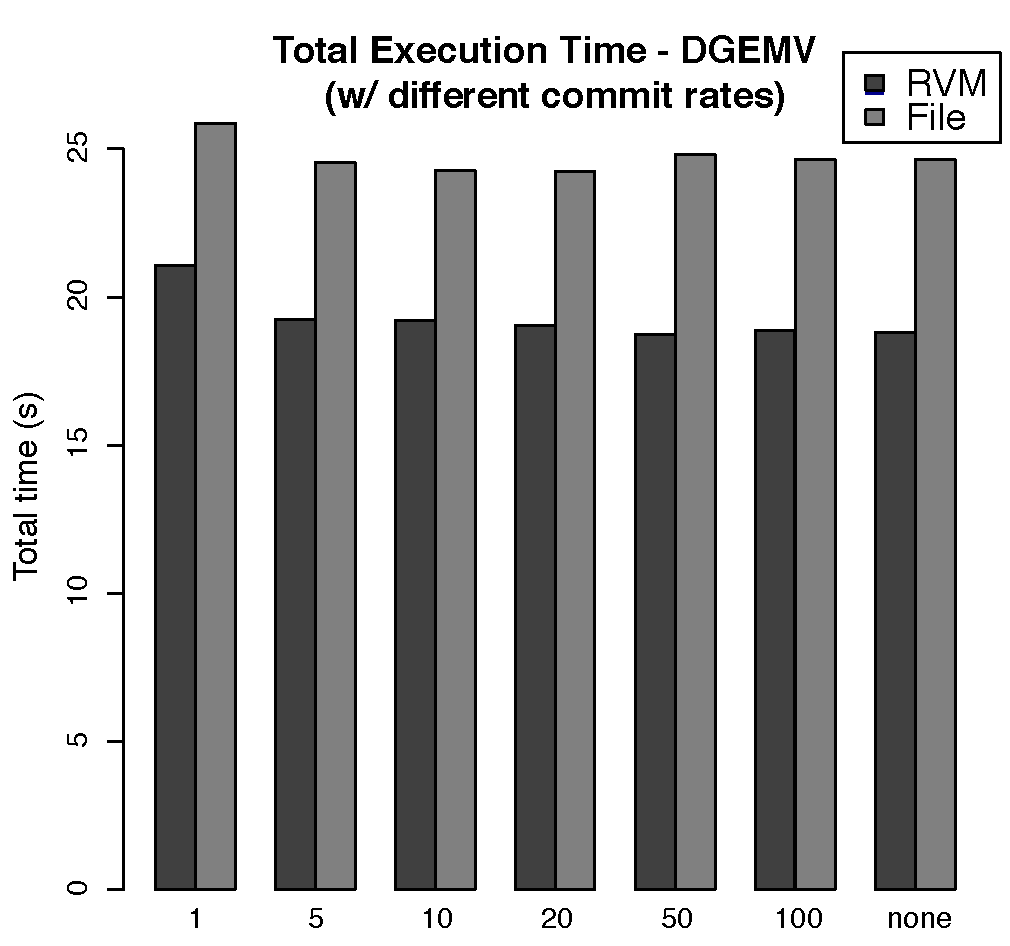
\includegraphics[scale=0.30]{dgemv_total_time_commit.pdf}
}
\end{center}
\caption{Total time of DGEMV application when committing at different rates}
\label{fig:dgemv_total_time_commit}
\end{figure}

\begin{figure}[t!]
\begin{center}
\resizebox{\columnwidth}{!}{%
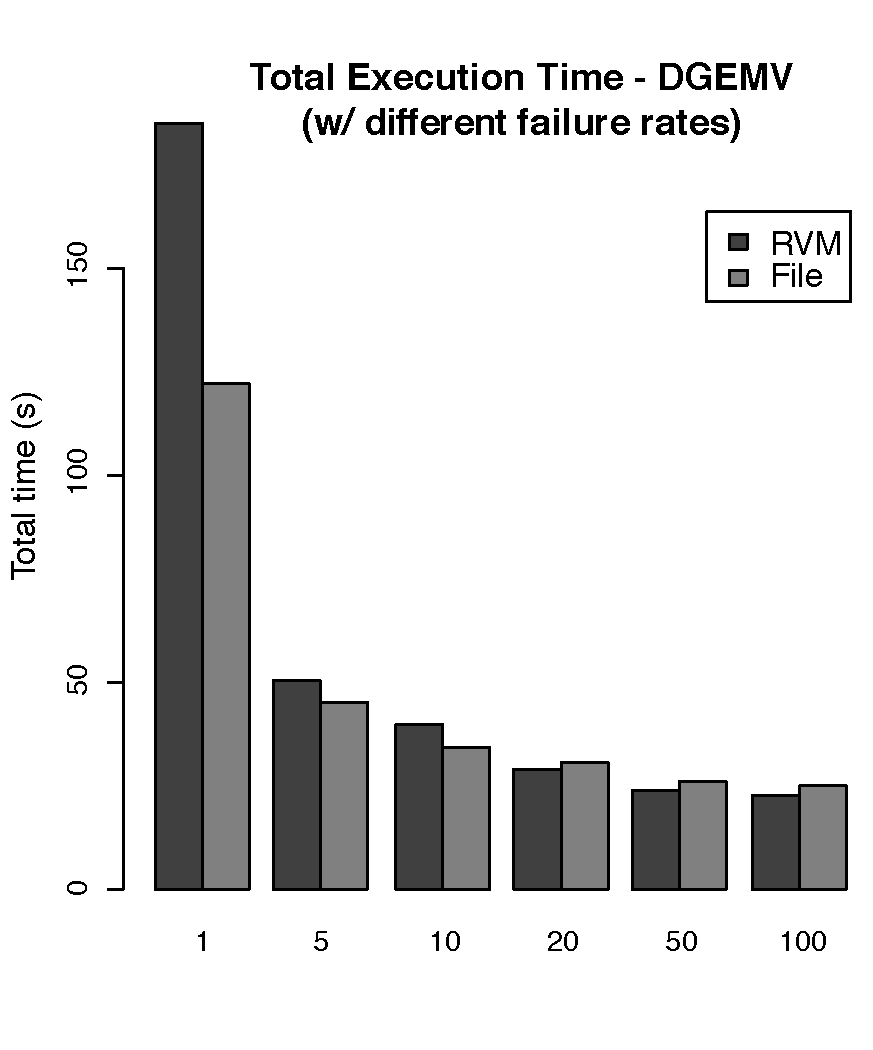
\includegraphics[scale=0.30]{dgemv_total_time_fail.pdf}
}
\end{center}
\caption{Total time of DGEMV application when failing/recovering at different rates}
\label{fig:dgemv_total_time_fail}
\end{figure}



\subsection{Gene Assembly}

% Genome Assembly
For a more complex benchmark, we ported the de novo genome assembly code that
was the basis of homework 3. This code involves the use of a large hash-table
(rough 100MB with our test input) as well as several linked-lists and other
complex data structures. In some ways, this is a best-case scenario for RVM. On
each checkpoint, only a fraction of the data is changed, and much of the memory
is constant (the input file). While we initially intended to implement a manual
serialization as we had done for DGEMV, it quickly became apparent that such an
undertaking would be almost as involved as writing the application in the first
place. We instead decided to compare it against a popular process-level
checkpointer called BLCR\cite{BLCR}. While DGEMV needed only to store the vector
and an iteration number, the genome assembly code was considerably more
complicated. Execution consists of two main phases. In the build phase, kmers
are read from a file and inserted into a hash table. The probe phase probes into
this hash table in order to construct the final contigs. To capture this
pattern, a global state structure was allocated from recoverable memory. This
global state stores shared structures such as the hash table and start-kmer
list, which phase is currently being executed (build or probe), and then
provides an opaque phase state pointer to be filled in by phase-specific code.
 The build phase keeps track of where in the input file it was, while probes
state is more complex. It needs to preserve which start-kmer it was
processing, where in the current contig it was, and where in the output file it
was writing. Each phase processed all 4 million kmers, for a total of 8 million
processing steps.

In figure \ref{fig:genome_total_time_commit} we vary the commit rate (in terms of number of
processing steps) from every 10 thousand (out of 8 million) up to 4 million
(one checkpoint per phase). At higher commit rates, RVM clearly outperforms
BLCR. In the exreme, RVM was able to complete in 800 seconds with a commit rate
of 10K, while we were forced to cancel the BLCR run after 30 minutes. Even at
more reasonable commit rates such as 1 million (8 commits), RVM was nearly twice
as fast as BLCR. It's only at the extreme low end of commit rates (4 million
and no commit) that BLCR was faster. This is because RVM pays a significant
up-front cost to allocate it's large recoverable state. Further analysis showed
that of the 10 seconds spent at a 4 million commit rate, a full 5s were spent
simply allocating memory, while build took only 2s and probe only 1s. This
clearly indicates a performance bottlenect in our system, although we do not
believe it is fundemental to the approach. See Section~\ref{sec:conclusion} for a
discussion of possible performance improvements. 

\begin{figure}[t!]
\begin{center}
%\resizebox{\columnwidth}{!}
\end{center}
\caption{Total time of genomic assembly application when committing at different rates. Total time when running BLCR at a rate of 10K is not shown}
\label{fig:genome_total_time_commit}
\end{figure}


\subsection{In-Memory Filesystem}

% In-Memory Filesystem


\section{Related Work}
\paragraph {\bf Virtual machine / Container checkpoint}
Systems such as~\ref{Tardigrade} or VMWare provide some level of fault-tolerance by checkpointing containers and virtual machines, respectively.
While these systems can checkpoint a program's data without knowing the program's internals they have limitations. 
First, using virtual machines incurs a performance overhead on applications. Secondly, checkpointing an entire virtual machine or container can be expensive.
We believe RVM provides an API that can be used to checkpoint only the data that matters to the user, and thus it can provide better performance with minimal developer effort.

\paragraph {\bf Key-value stores and DBMSs}
Key-value stores such as RAMCloud and DBMSs such as Postgres can be used to store a program's data to remote nodes and provide similar
properties as RVM. While we believe that many of the techniques and lessons used in these systems can be applied in RVM, we think these 
systems are not a good fit for the applications we envision using with RVM.
First, most modern key-value stores do not provide atomic multi-key writes.
Secondly, the API provided by key-value stores despite being simple is not suitable for virtual memory replication.
Likewise, DBMSs sacrifice data access latency in favour of many features that are not required in this context while. Additionally, the schema model required by traditional DBMSs is
does not fit well with arbitrarily-sized regions of memory.


\paragraph {\bf Virtual memory replication}
Systems like Mojim~\cite{Mojim} or LRVM~{LRVM} can be used to replicate virtual memory.

%
%\section{Conclusion and Future Work}
%In this paper, we presented Recoverable Virtual Memory, our solution for easy
replication and recovery of application state. We have attempted to provide our
implementation with features we believe are highly desirable for the
application programmer, such as a simple and understandable API; restoration of
virtual address locations, which allows for recovery of complex data structures
without the need for serialization; and reasonably low overhead.  Of these
three goals, we have accomplished the first two, but there is still
considerable work to be done in regards to performance.

The most obvious optimization we could make is to coalesce RDMA operations for
contiguous pages. In our current infiniband backend, allocation of the backing
memory for multiple contiguous pages must be done a page at a time.  However,
it would be much more efficient to perform a single contiguous allocation on
the server side. That way, the number of RDMA write calls and TXN\_MULTI\_CP
messages does not need to increase as the number of pages increases. There are
probably other areas for performance improvement that we could discover through
more intensive profiling of the benchmark programs.

Another avenue we could explore are alternative backends for the RMEM layer.
There are various networking and non-volatile memory technologies that we could
investigate, such as SSDs and RDMA over Converged Ethernet. We could also
implement different consistency semantics to explore the tradeoffs of
performance and consistency.

Finally, we would like to integrate RVM with existing runtimes and recovery
frameworks to provide a more complete data replication and recovery solution.

The complete code for our RVM implementation is available on GitHub at
https://github.com/zhemao/rmem-server.


%%%%%%%%%%%%%%%%%%%%%%%%%%%%%%%%%%%%%%%%%%%%%%%%%%%%%%%%%%%%%%%%%%%%%%%%%%%%%%%%
% \pagebreak
\bibliography{main}
\bibliographystyle{abbrv}

\end{document}
